\documentclass[a4paper]{article}

\usepackage[english]{babel}
\usepackage[utf8]{inputenc}
\usepackage{graphicx}
\usepackage{enumitem}
\usepackage{blindtext}

\usepackage{karnaugh-map}

\graphicspath{ {./images/} }
    
\title{CE2210, Sec. 3 \\Homework 3}
\author{Evan Wilcox}
\setlength\parindent{0pt}
    
\date{Due March 6, 2019}
    
\begin{document}
    \maketitle

    \begin{enumerate}
        
        \item $F = AB + C$ \\ 
        
        \begin{tabular}{ c|c }
            $ABC$ & $F$ \\ \hline
            000 & 0 \\
            001 & 1 \\
            010 & 0 \\
            011 & 1 \\ \hline
            100 & 0 \\
            101 & 1 \\
            110 & 1 \\
            111 & 1 \\
        \end{tabular} \\

        CSOP: $F = (\bar{A}\bar{B}C) + (A\bar{B}\bar{C}) + (A\bar{B}C) + (AB\bar{C}) + (ABC)$ \\
        Minterm: $F=\Sigma m(1, 3, 5, 6, 7)$ 

        \vspace{2em}

        \item $F = AB + BC$ \\ 
        
        \begin{tabular}{ c|c }
            $ABC$ & $F$ \\ \hline
            000 & 0 \\
            001 & 0 \\
            010 & 0 \\
            011 & 1 \\ \hline
            100 & 0 \\
            101 & 0 \\
            110 & 1 \\
            111 & 1 \\
        \end{tabular} \\

        CPOS: $F = (A+B+C) \cdot (A+B+\bar{C}) \cdot (A+\bar{B}+C) \cdot (\bar{A}+B+C) \cdot (\bar{A}+B+\bar{C})$ \\
        Maxterm: $F=\Sigma M(0, 1, 2, 4, 5)$ \\

        \item $F = AB + BC + AC$ \\
        $= AB(C+\bar{C}) + BC(A+\bar{A}) + AC(B+\bar{B})$ (Compliment) \\
        $= (ABC + AB\bar{C}) + (ABC + \bar{A}BC) + (ABC + A\bar{B}C)$ (Distribute) \\ 
        $= ABC + AB\bar{C} + \bar{A}BC + A\bar{B}C)$ (Idempotence)


        \newpage
        \item AND-OR PLA
        \begin{center}
            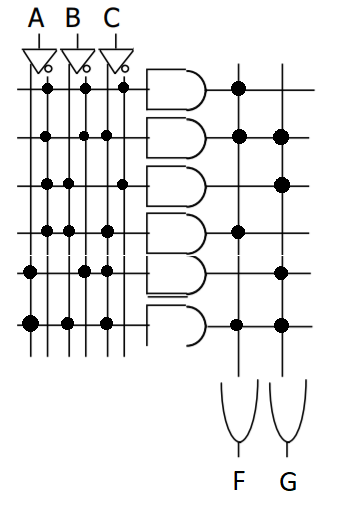
\includegraphics[scale=0.8]{4}
        \end{center}

        \item OR-AND PLA 
        \begin{center}
            %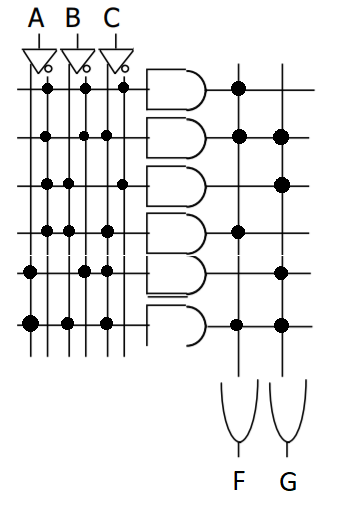
\includegraphics[scale=0.8]{4}
        \end{center}

        \vspace{7cm}
        \item
        \begin{enumerate}
        
            \item $425_{10}$ = 0100 0010 $0101_{BCD}$
        
            \item $17_{10}$ = 0001 $0111_{BCD}$
        
            \item $2039_{10}$ = 0010 0000 0011 $1001_{BCD}$
        
        
        \end{enumerate}

        \newpage
        \item 
        \begin{enumerate}
            \item C function.\\
            \begin{karnaugh-map}*[4][4][1][$CD$][$AB$]
                \minterms{0, 1, 3, 4, 5, 6, 7, 8, 9}
                \maxterms{2}
                \indeterminants{10, 11, 12, 13, 14, 15}
                \implicant{0}{9}
                \implicant{1}{11}
                \implicant{4}{14}
                \implicantedge{2}{2}{10}{10}
            \end{karnaugh-map} 

            MSOP: $F = B + \bar{C} + D$ \\ 
            MPOS: $F = B + \bar{C} + D$ \\
            
            \vspace{6em}

            \item D function \\
            \begin{karnaugh-map}*[4][4][1][$CD$][$AB$]
                \minterms{0, 2, 3, 5, 6, 8}
                \maxterms{1, 4, 7, 9}
                \indeterminants{10, 11, 12, 13, 14, 15}
                \implicantedge{3}{2}{11}{10}
                \implicant{2}{10}
                \implicant{5}{13}
                \implicantcorner
                \implicantedge{1}{1}{9}{9}
                \implicant{4}{12}
                \implicant{7}{15}
            \end{karnaugh-map}
        
            MSOP: $F = \bar{B}\bar{D} + B\bar{C}D + \bar{B}C + C\bar{D}$ \\ 
            MPOS: $F = (\bar{B}+C+D) \cdot (B+C+\bar{D}) \cdot (\bar{B}+\bar{C}+\bar{D})$ 

        \end{enumerate}
        
        
        \newpage
        \item
        \begin{enumerate}

            \item $f(x,y,z) = \Sigma m(0,1,2,3,4,6,7)$ \\
            \begin{karnaugh-map}*[4][2][1][$YZ$][$X$]
                \minterms{0,1,2,3,4,6,7}
                \maxterms{5}
                \implicantedge{0}{4}{2}{6}
                \implicant{0}{2}
                \implicant{3}{6}

                \implicant{5}{5}
            \end{karnaugh-map}

            MSOP: $F = \bar{X} + \bar{Z} + Y$ \\
            MPOS: $F = \bar{X} + \bar{Z} + Y$

            \vspace{10em}
 

            \item $f(w,x,y,z) = \Sigma m(1,3,4,6,7,9,11,13,15)$ \\ 
            \begin{karnaugh-map}*[4][4][1][$YZ$][$WX$]
                \minterms{1,3,4,6,7,9,11,13,15}
                \maxterms{0, 2, 5, 8, 10, 12, 14}
                \implicantedge{4}{4}{6}{6}
                \implicant{13}{11}
                \implicantedge{1}{3}{9}{11}
                \implicant{3}{11}

                \implicantedge{0}{0}{8}{8}
                \implicant{12}{8}
                \implicantedge{2}{2}{10}{10}
                \implicant{14}{10}
                \implicant{5}{5}
            \end{karnaugh-map}

            MSOP: $F = \bar{W}X\bar{Z} + WZ + \bar{X}Z + YZ$ \\
            MPOS: $F = (\bar{W}+Y+Z) \cdot (X+Y+Z) \cdot (\bar{W}+\bar{Y}+Z) \cdot (X+\bar{y}+Z) \cdot (W+\bar{X}+Y+\bar{Z})$

        \end{enumerate}


    \end{enumerate}





\end{document}